\documentclass[10pt,a4paper]{report}
\usepackage[utf8]{inputenc}
\usepackage{amsmath}
\usepackage{amsfonts}
\usepackage{amssymb}
\usepackage{graphicx}
\usepackage{lmodern}
\usepackage[left=2cm,right=2cm,top=2cm,bottom=2cm]{geometry}

\begin{document}

\author{Yapi Donatien Achou}
\title{Project report }
\maketitle

\section{Introduction}
We solve the wave equation with the finite difference method. The model equation is discretised using a second order scheme. for validation, the numerical solution is compared with a constant solution, a plug wave and a manufactured solution respectively. Convergence test with the manufactured solution did not recover the convergence rate of 2 due to an implemetation error.

\section{Mathematical equation}
we solve the wave equation:
\begin{equation}\label{main}
\frac{\partial^{2} u}{\partial t^{2}} +b\frac{\partial u}{\partial t}  +\frac{\partial}{\partial x}\left(  q(x,y)\frac{\partial}{\partial x}   \right) +\frac{\partial}{\partial y}\left(  q(x,y)\frac{\partial}{\partial y}   \right) +f(x,y,t)
\end{equation}

with boundary condition:
\begin{equation}
\frac{\partial u}{\partial n} = 0
\end{equation}

and initial condition:
\begin{equation}
\frac{\partial u(x,y,0)}{\partial t} = V(x,y)
\end{equation}

\begin{equation}
u(x,y,0) = I(x,y)
\end{equation}

where $b$ is the damping factor, $q(x,y)$ is the wave velocity and f is the source term.

\section{Numerical scheme and discretisation}
by using a second order scheme we obtained the following discretisation for the time derivative and the spatial derivative:
 
\begin{equation}\label{t2}
\frac{\partial^{2} u}{\partial t^{2}} \approx \frac{ u_{i,j}^{n+1}-2u_{i,j}^{n}+u_{i,j}^{n-1}}{\delta t^{2}} 
\end{equation} 

\begin{equation}\label{t1}
b\frac{\partial u}{\partial t} \approx b\frac{ u_{i,j}^{n+1}-u_{i,j}^{n-1}}{2\Delta t} 
\end{equation} 

\begin{equation}\label{x2}
\frac{\partial}{\partial x}\left(  q(x,y)\frac{\partial}{\partial x}   \right) \approx \frac{ (q_{i,j}+q_{i+1,j})(u_{i+1,j}^{n}- u_{i,j}^{n})-(q_{i,j}+q_{i-1,j})(u_{i,j}^{n}-u_{i-1,j}^{n}) }{2\Delta x^{2}} = D_{xx}
\end{equation}

\begin{equation}\label{y2}
\frac{\partial}{\partial y}\left(  q(x,y)\frac{\partial}{\partial y}   \right) \approx \frac{ (q_{i,j}+q_{i,j+1})(u_{i,j+1}^{n}- u_{i,j}^{n})-(q_{i,j}+q_{i,j-1})(u_{i,j}^{n}-u_{i,j-1}^{n}) }{2\Delta y^{2}}=D_{yy}
\end{equation}

Inserting \ref{t2},\ref{t1},\ref{x2} and \ref{y2} into \ref{main} we obtain the general scheme for $i,j = 1,...,N_{x}$:

\begin{equation}\label{mains}
u_{i,j}^{n+1} = k_{1}u_{i,j}^{n-1}+k_{2}u_{i,j}^{n}+k_{3}(\Delta_{i,j}^{n}+f_{i,j}^{n})
\end{equation}

with 
\begin{equation}
k_{1} = \frac{ \frac{\Delta t b}{2} -1 }{\frac{\Delta t b}{2} +1 }\nonumber
\end{equation}

\begin{equation}
k_{2} = \frac{ 2}{\frac{\Delta t b}{2} +1 }\nonumber
\end{equation}

\begin{equation}
k_{3} = \frac{ \Delta^{2}}{\frac{\Delta t b}{2} +1 }\nonumber
\end{equation}

\begin{equation}
\Delta = Dxx + Dyy\nonumber
\end{equation}

To find the modified scheme for the first time step we use the Initial condition:
\begin{equation}
\frac{\partial u(x,y,0)}{\partial t} \approx \frac{ u_{i,j}^{n+1}-u_{i,j}^{n-1}}{2\Delta t}  = V \nonumber
\end{equation}

solving for $u_{i,j}^{n-1}$ and inserting it in \ref{mains} we get for
 $i,j = 1,...,N_{x}$ and $n=0$:
 
 \begin{equation}\label{fi}
 u_{i,j}^{n+1} = r_{1}+r_{2}u_{i,j}^{n}+r_{3}(\Delta +f_{i,j})
 \end{equation}
 
 with 
 \begin{equation}
 r_{1} = \frac{2k_{1}\Delta t V_{i,j}^{n}}{k_{1}-1} \nonumber
 \end{equation}
 
 \begin{equation}
 r_{2} = \frac{k_{2}}{1-k_{1}}\nonumber
 \end{equation}
 
 \begin{equation}
 r_{3} = \frac{k_{3}}{1-k_{1}}\nonumber
 \end{equation}
 
 The boundary points for the first time step and the subsequent time are calculated by using the boundary condition:
 \begin{equation}
\frac{\partial u}{\partial x} \approx  \frac{ u_{i,j}^{n+1}-u_{i,j}^{n-1}}{2\Delta x}  = 0 \nonumber
\end{equation}

\begin{equation}
\frac{\partial u}{\partial y} \approx  \frac{ u_{i,j}^{n+1}-u_{i,j}^{n-1}}{2\Delta y}  = 0 \nonumber
\end{equation}

\begin{equation}
\frac{\partial q}{\partial x} \approx  \frac{ u_{i,j}^{n+1}-u_{i,j}^{n-1}}{2\Delta x}  = 0 \nonumber
\end{equation}

\begin{equation}
\frac{\partial q}{\partial y} \approx  \frac{ u_{i,j}^{n+1}-u_{i,j}^{n-1}}{2\Delta y}  = 0 \nonumber
\end{equation}
so that for $i=0$
\begin{equation}\label{i0}
u_{i-1,j}^{n} = u_{i+1,j}^{n} 
\end{equation}
for $j=0$
\begin{equation}\label{j0}
u_{i,j-1}^{n} = u_{i,j+1}^{n} 
\end{equation}
for $i=N_{x}$
\begin{equation}\label{in}
u_{i+1,j}^{n} = u_{i-1,j+1}^{n} 
\end{equation}
for $j=N_{y}$
\begin{equation}\label{jn}
u_{i,j+1}^{n} = u_{i,j-1}^{n} 
\end{equation}
equation \ref{fi} with \ref{i0}, \ref{i0}, \ref{in},\ref{jn} are used to calculate the boundary points for the forst time step while
equation \ref{mains} with \ref{i0}, \ref{i0}, \ref{in},\ref{jn} are used to calculate the boundary points for subsequent time

\section{Numerical result and validation}
The constant solution and plug wave gives good result when comparing the numerical solution with exact constant solution. However for manufacture solution the error is too large. To prove that the numerical method is correctly implemented despite the relatively large error found with the manufactured solution, a convergence test is carried out as followed:
The numerical scheme is of order $p$ such that 

\begin{equation}
E = \frac{C}{\Delta t^{p}} \nonumber
\end{equation}b
where E is the error between the manufactured solution and the numerical solution. $C$ is a constant depending on the manufactured. By varying the time step $\Delta t$ and finding the corresponding error $E$ we get

\begin{equation}\label{cr}
p = \frac{ log(E_{i}/E_{i+1})}{log(\Delta t_{i+1}/ \Delta t_{i})}
\end{equation}

Applying \ref{cr} we did not recover a convergence rate of 2.

\section{Solution with different Initial condition}

\begin{figure}[h!]
  \caption{propagating wave at $t=0.1$ with constant parameters}
  \centering
    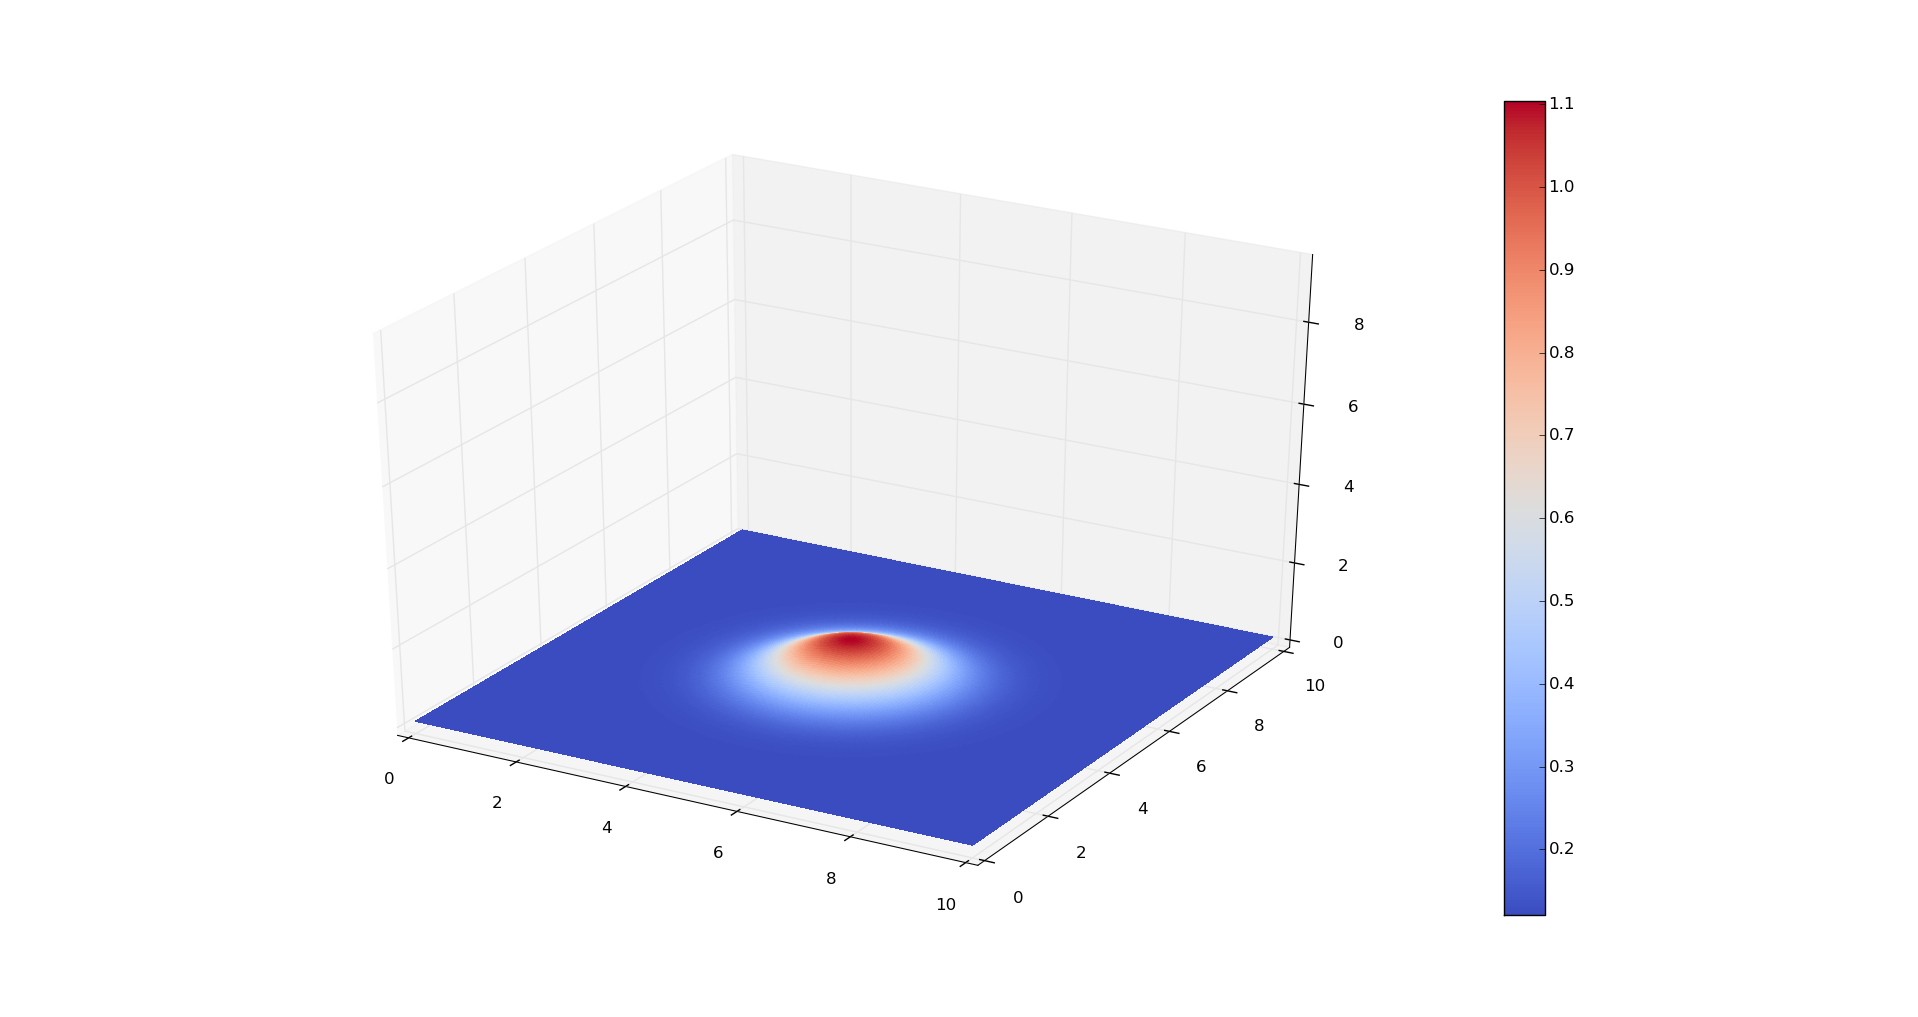
\includegraphics[width=1.5\textwidth]{t01.png}
\end{figure}

\begin{figure}[h!]
  \caption{propagating wave at $t=2$ with constant parameters}
  \centering
    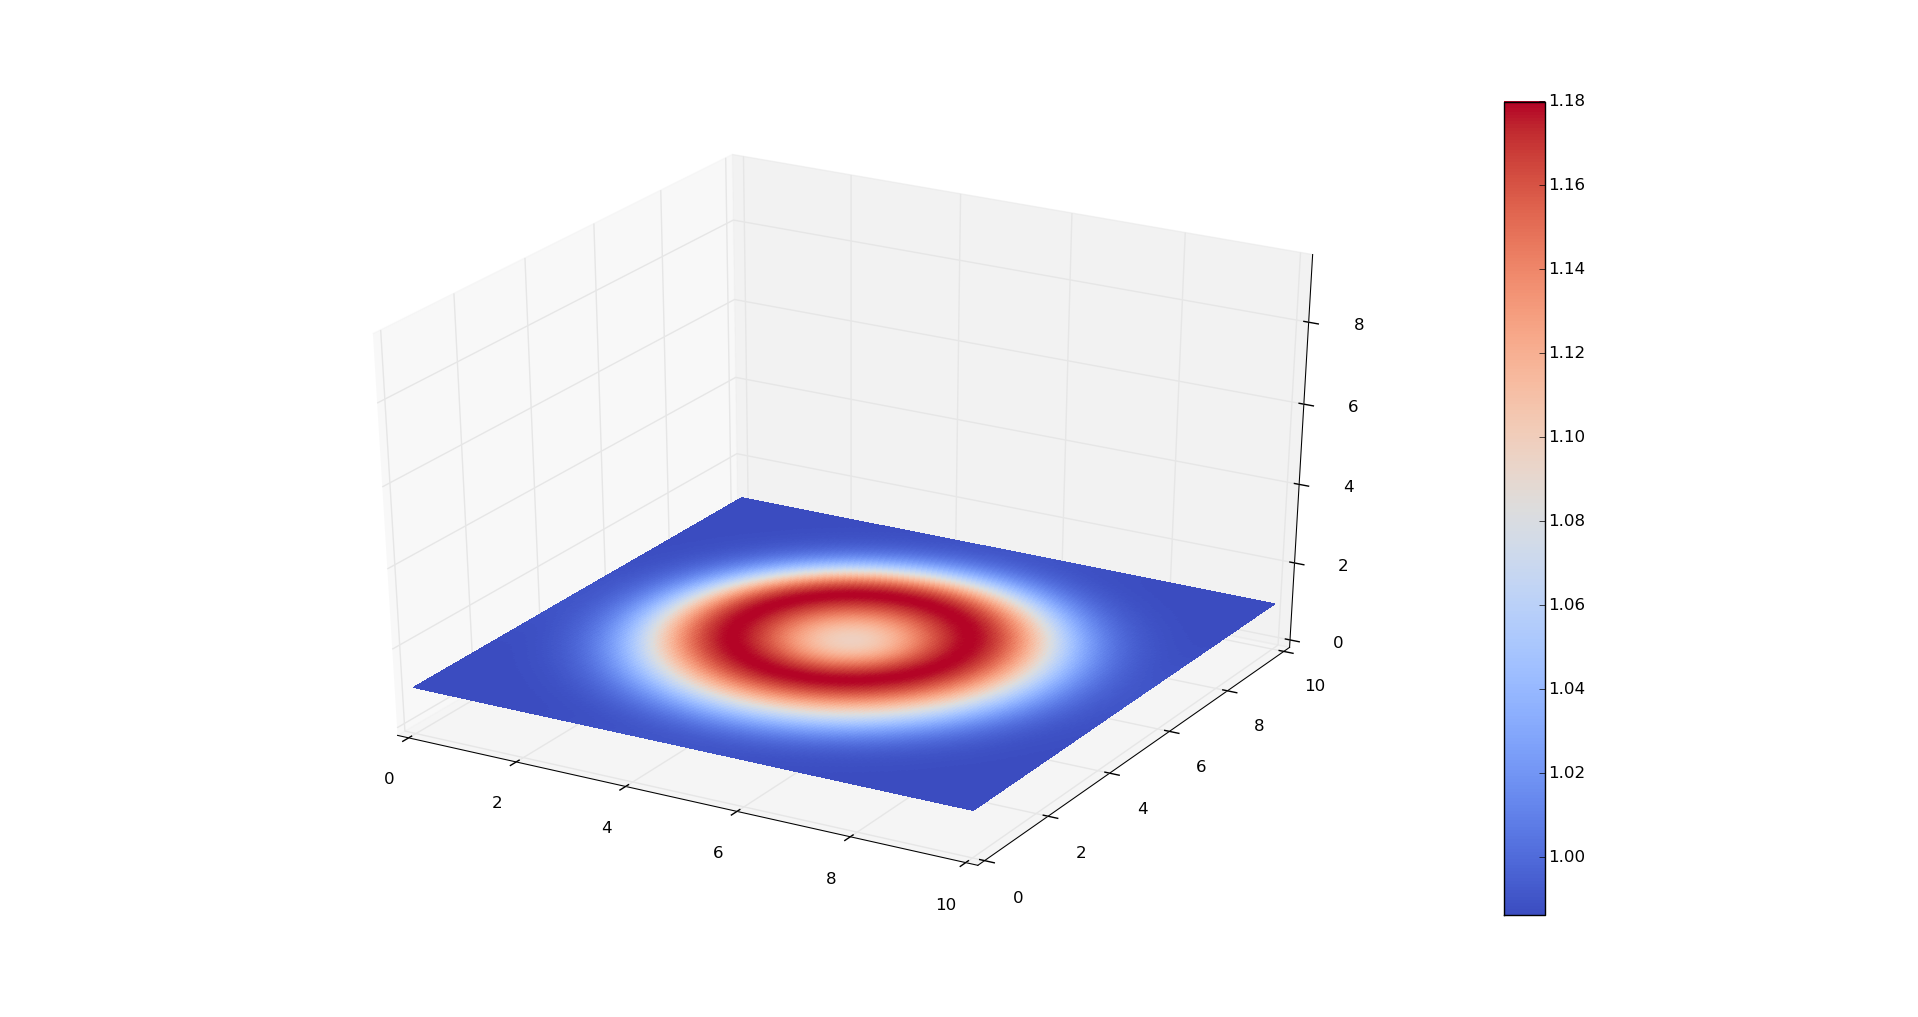
\includegraphics[width=1.5\textwidth]{t2.png}
\end{figure}

\begin{figure}[h!]
  \caption{propagating wave at $t=3$ with constant parameters}
  \centering
    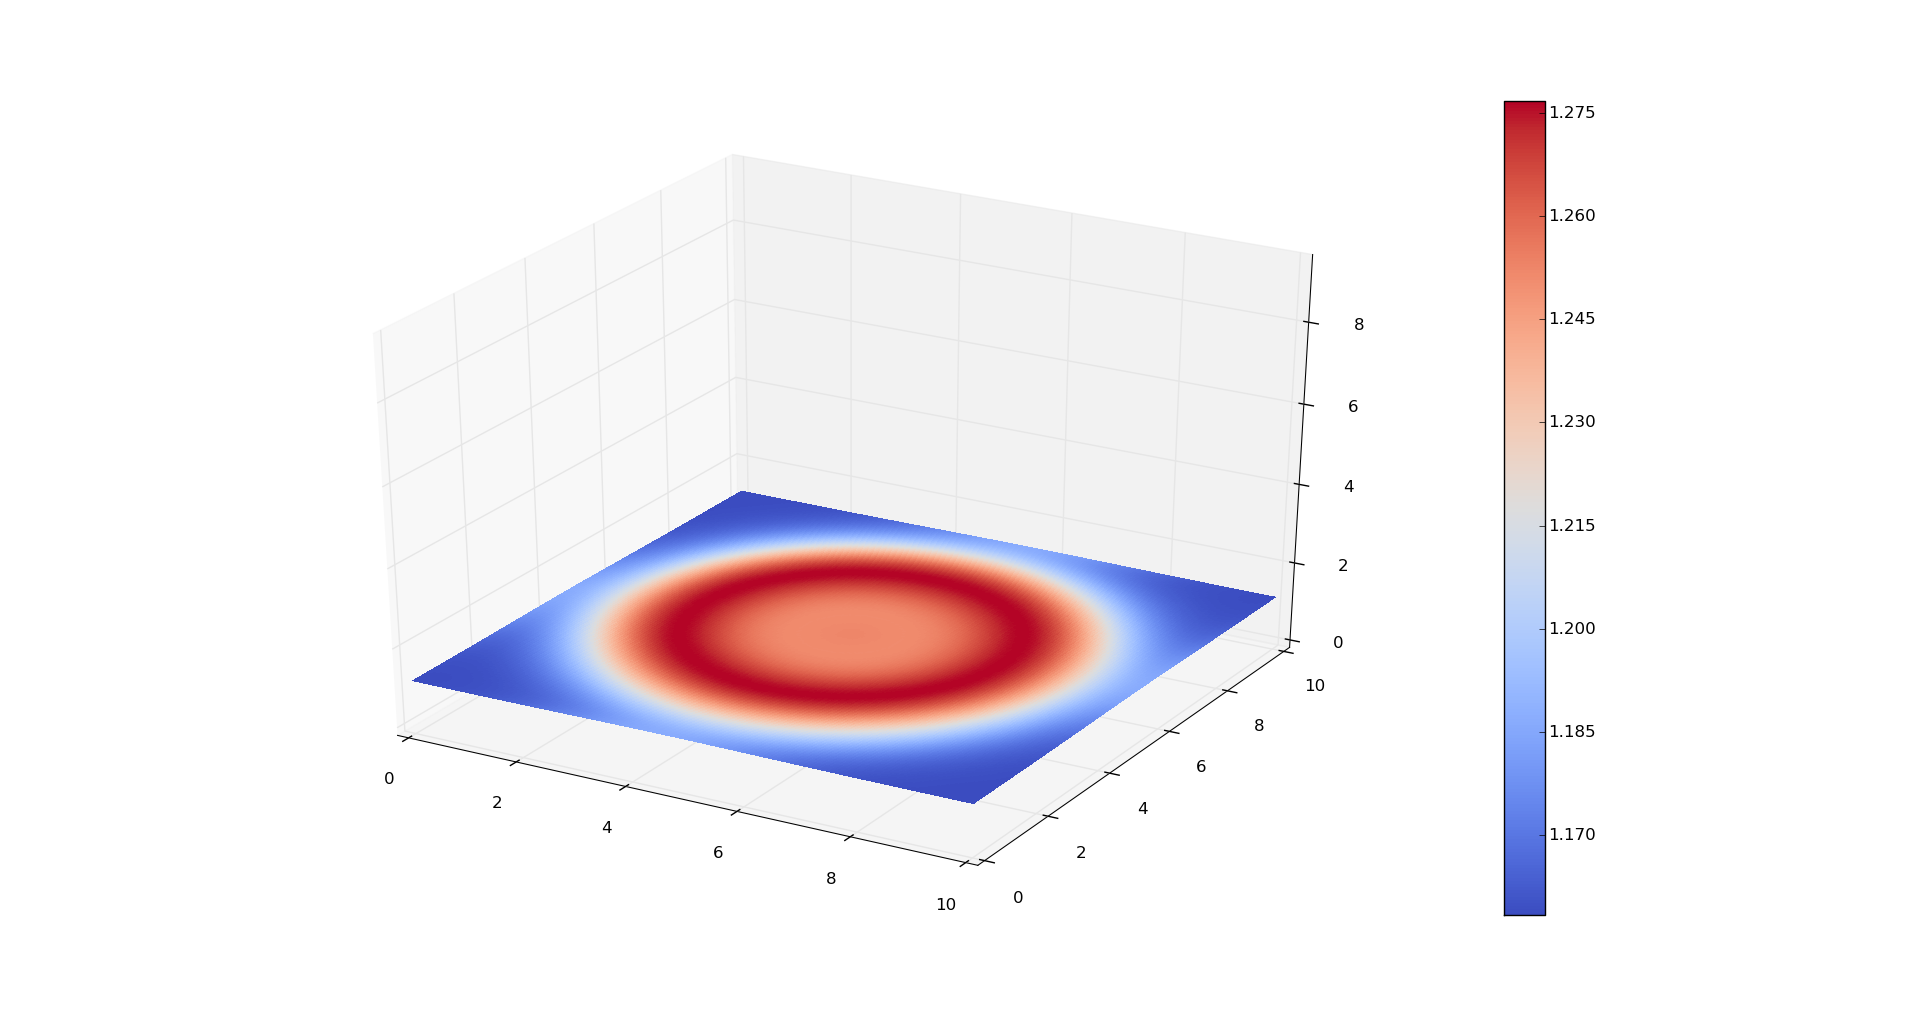
\includegraphics[width=1.5\textwidth]{t3.png}
\end{figure}

\begin{figure}[h!]
  \caption{propagating wave at $t=4$ with constant parameters}
  \centering
    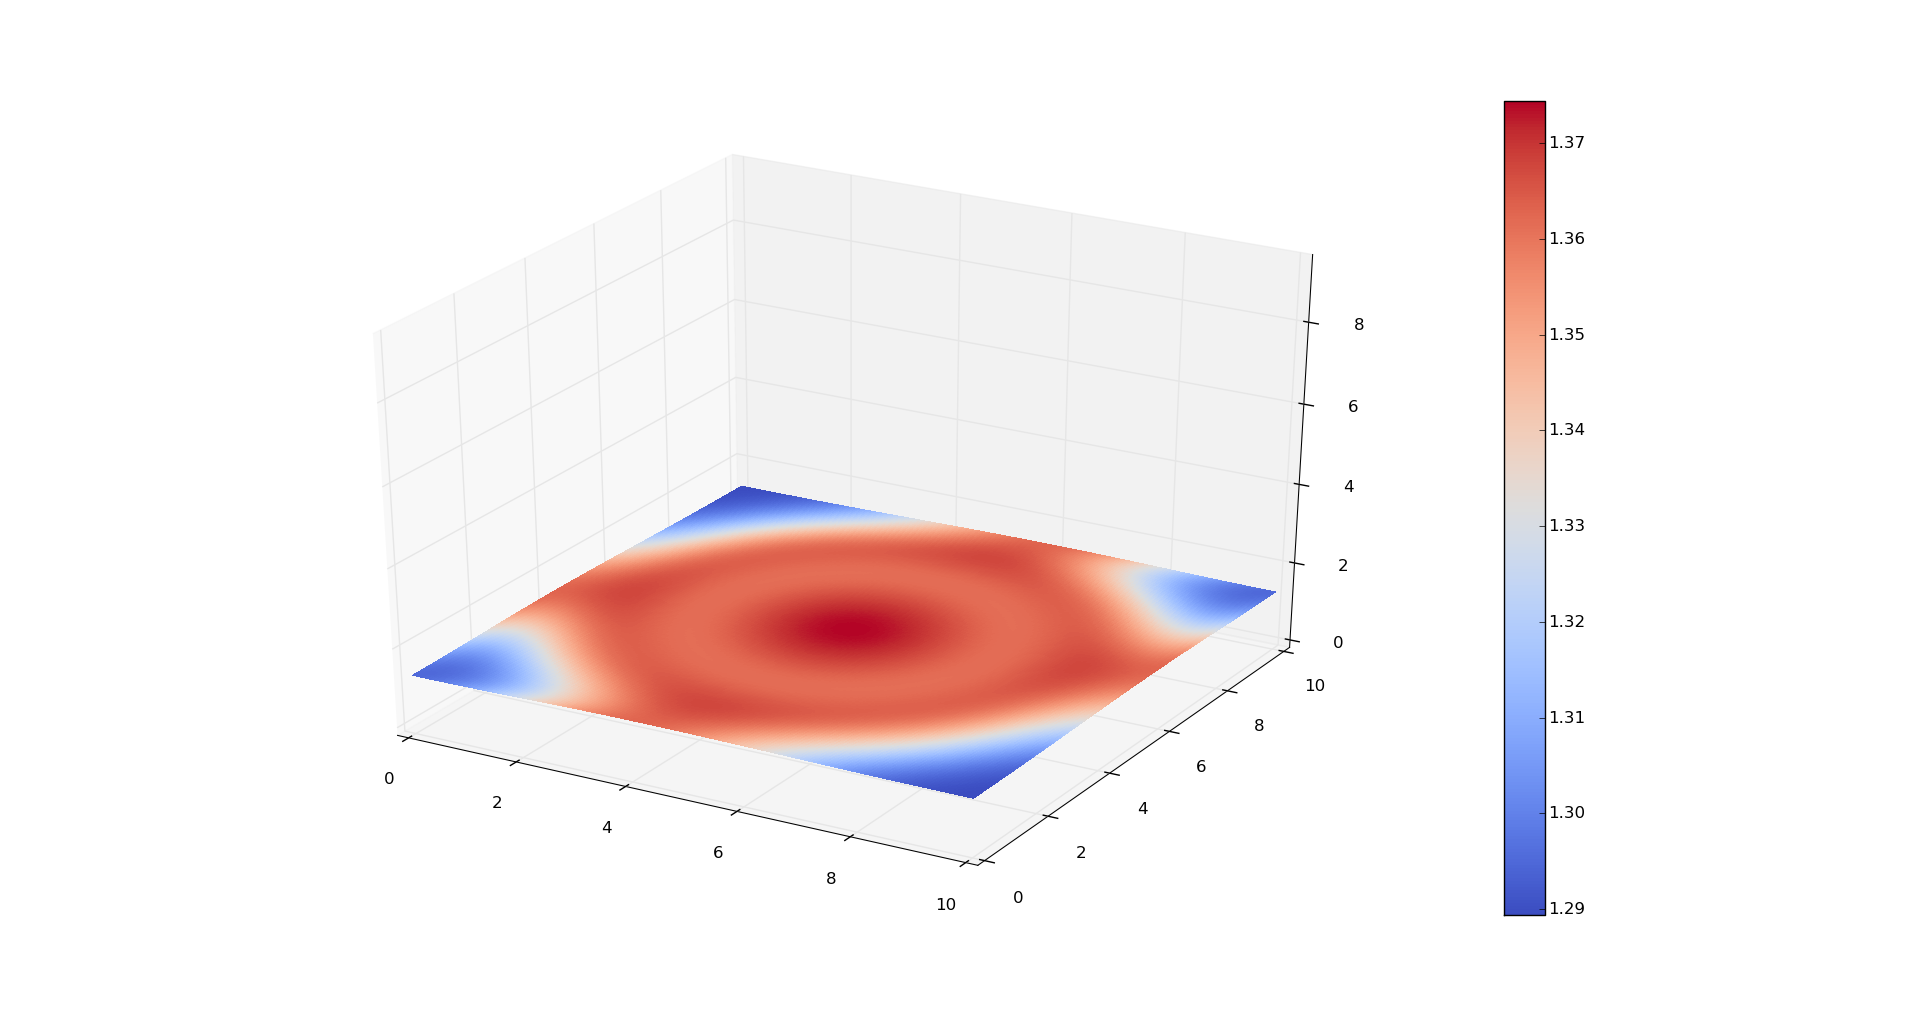
\includegraphics[width=1.5\textwidth]{t4.png}
\end{figure}

















\end{document}